\chapter{Formulation}
The Arbitrary Lagrangian-Eulerian (ALE) Formulation is the modelling technique to couple/decouple the motion of particles or bodies in the Eulerian and Lagrangian Formulation. The formulation is commonly employed in Fluid-Structure Interaction Problems, where the domain of the solid is affected by the fluid and, the other way round \cite{ALE_FSI}. The key feature about ALE formulation is the decomposition of the body's motion as the motion of Eulerian frames and the respective Lagrangian domains. The method to perform decomposition of motion is described in section \ref{ALE_Description}.
\section{General Description}
\label{ALE_Description}
Let the fixed Eulerian reference frame be defined by $\chi$; further, the corresponding Lagrangian domain be $\mathbf{R}_{\chi}$, then it is possible to define the initial state of the body with $(\mathbf{R}_{\chi}, \chi)$. Similarly, let the final state of the body be $(\mathbf{R}_{\mathbf{x}}, \mathbf{x})$ and $\boldsymbol{\Phi}$ the transformation from the state $(\mathbf{R}_{\chi}, \chi)$ to $(\mathbf{R}_{\mathbf{x}}, \mathbf{x})$. Then the ALE formulation constructs an intermediate state $(\mathbf{R}_{\mathbf{X}}, \mathbf{X})$, which represents the change in the Lagrangian domain with respect to the initial state, keeping the Eulerian frame constant. It is possible to construct a Lagrangian state transformation $\Psi$, which transforms the system from the initial state to the intermediate state. In addition to this, the Eulerian transformation that transforms the system from the intermediate state to the final state can be given by $\varphi$. The ALE model transforms the system from the initial state to the final state transitioning through the intermediate state, as shown in \autoref{fig:ALEdomain} \cite{ALE}, then the relationship \autoref{eq:ALE_Transformation} holds.
% Let us assume that we have a fixed Eulerian reference frame $\chi$ and Lagrangian domain $\mathbf{R}_{\chi}$ describing the initial state of the body. Further let us assume that the final state of the body is defined by the state $(\mathbf{R}_{\mathbf{x}}, \mathbf{x})$. Also let us consider $\Phi$ be the transformation that takes system from state $(\mathbf{R}_{\chi}, \chi)$ to $(\mathbf{R}_{\mathbf{x}}, \mathbf{x})$. In the ALE formulation we can describe the transformation of the body from the initial state to the final state using an intermediate state $(\mathbf{R}_{\mathbf{X}}, \mathbf{X})$. The intermediate state represents the change in the Lagrangian domain with respect to the initial state, keeping the Eulerian frame constant. Then the final state of the body can be reached from the intermediate state using a transformation say $\varphi$, as shown in the figure \ref{fig:ALEdomain}. This is results in the following set of equations \cite{ALE}.
\begin{equation}\label{eq:ALE_Transformation}
     \boldsymbol{\Phi} = \boldsymbol{\Psi} \circ \boldsymbol{\varphi}
\end{equation}

\begin{figure}[!ht]
    \centering
    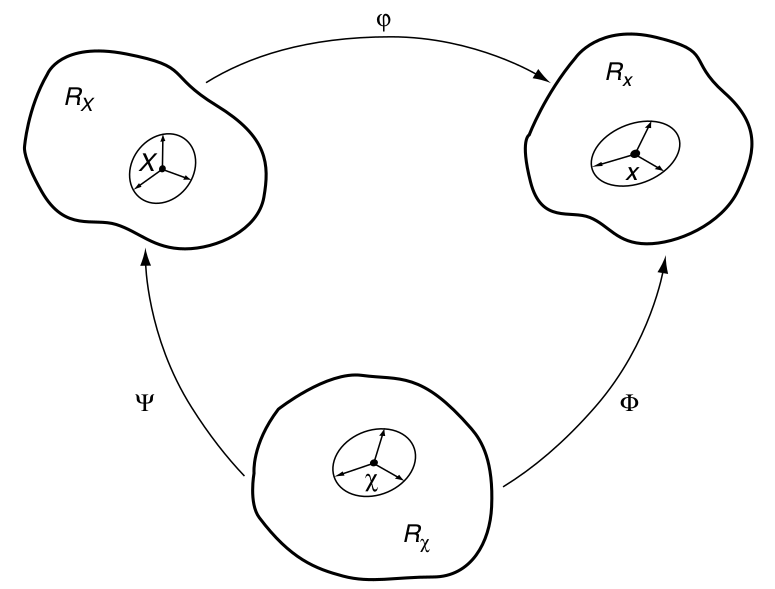
\includegraphics[width=0.5\textwidth]{Domains}
    \caption{The motion the body in the ALE formulation. The axes $\chi, \mathbf{X}$ and $\mathbf{x}$ represent the Eulerian frame in the body. While the $\mathbf{R}_{\chi}, \mathbf{R}_{\mathbf{X}}$ and $\mathbf{R}_{\mathbf{x}}$ represent the Lagrangian domain. The Final state of the body is represented by $\mathbf{R}_{\mathbf{x}}, \mathbf{x}$, which can be obtained by Lagrangian transformation $\Psi$ with respect to fixed system $\mathbf{R}_{\chi}, \chi$ and then Eulerian transformation $\varphi$ with respect to $\mathbf{R}_{\mathbf{X}}, \mathbf{X}$.}
    \label{fig:ALEdomain}
\end{figure}

\section{Vehicle Model}
\subsection{Model Assumption}
\label{subsection:ALEModelAssumption}
This formulation uses the same physical model, as described in section \ref{subsection:Vehicle_Model}, with the following assumptions made to address the performance issues posed in the MBD formulation, as described in section \ref{MBD_limit}. \par
\begin{enumerate}
    \item The torsional springs at the wheels and the main body were removed.
    \item The wheels and tyres were constrained to be vertically below the corner of the main body at all times.
    \item The moment of inertia of the main body remains constant which implies the angle of rotation for the centre of gravity are small.
\end{enumerate}
The aforementioned assumptions result in a formulation where the horizontal motion of the vehicle is independent of the vertical motion while the vertical motion is still impacted due to the rotational components arising from the horizontal force. The resulting physical system is shown in figure \ref{fig:ALEstick}. It is worth noting the differences between the model described in section \ref{subsection:MBDPhysicalDescription} and Figure \ref{fig:ALEstick}. \par
%Add ALE pic here%
\begin{figure}[!ht]
    \centering
    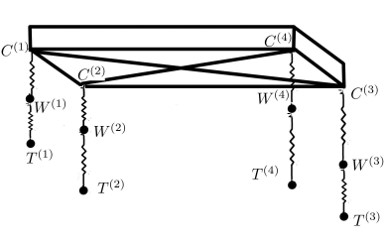
\includegraphics[width=0.45\textwidth]{ALE_stick_diagram}
    \caption{Resulting Physical system with the assumptions taken in account for ALE modelling.}
    \label{fig:ALEstick}
\end{figure}

\noindent An illustrative example of Lagrangian-Eulerian frame is given by the circular motion of the vehicle, represented in \ref{fig:Eg_Lagrangian_Eulerian_Circular}. As well, by this figure we introduce the notations for $x$, $y$ and $z$ axes, the $z$ axis being oriented downwards with respect to centre of mass and the main motion of the vehicle in the $X-Y$ plane. 

\begin{figure}[!ht]
    \centering
    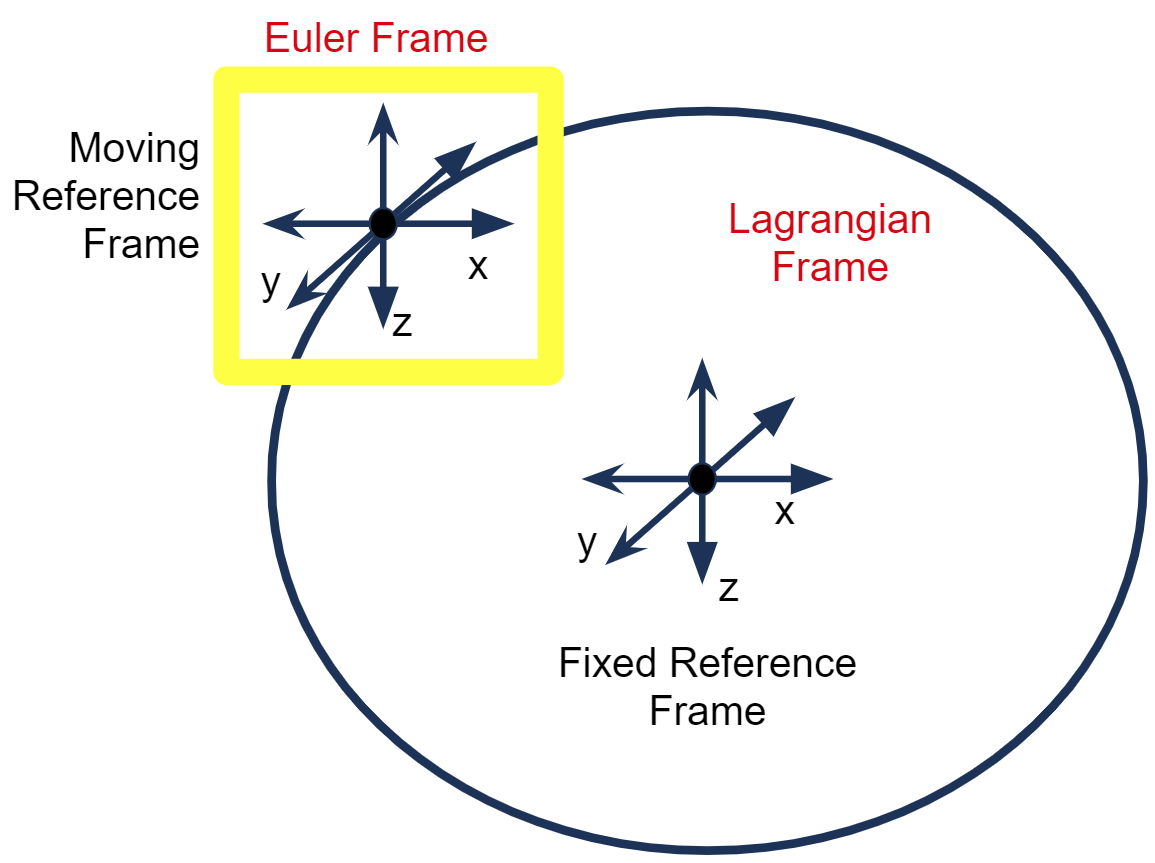
\includegraphics[width=0.45\textwidth]{Eg_Lagrangian_Eulerian_Circular}
    \caption{Example of Lagrangian-Eulerian frame for uniform circular motion}
    \label{fig:Eg_Lagrangian_Eulerian_Circular}
\end{figure}

\subsection{Model Formulation}
\label{subsection:ALEModelFormulation}
The considerations made in section \ref{subsection:ALEModelAssumption} allow for a reduction in translational degrees of freedom along the $X-Y$ axes to two, which are the $X-Y$ coordinates of the centre of gravity of the main body. Additionally, the overall rotational degree of freedom is also reduced along the $Z$ axis to one, being the rotation of the main body. The coordinates of the other eight components can be evaluated by the constraint equations. The resulting simplified system was used as the Lagrangian domain. Since the horizontal motion of the body is not affected by the vertical motion, the Lagrangian frame was constrained to move in the $X-Y$ plane. This results in a reduced system having only three degrees of freedom describing the Lagrangian state of the vehicle, and can be written in the following form. \par
\begin{equation}
     \mathbf{R}_{\phi} = \begin{pmatrix} 
                        X_{\phi} \\
                        Y_{\phi} \\
                        \theta_{\phi}
                        \end{pmatrix},
\end{equation}
where:
\begin{itemize}
    \item $\mathbf{R}_{\phi}$: State vector of Lagrangian Domain.
    \item $X_{\phi}$: $X$ coordinate of the Centre of Gravity of the main body.
    \item $Y_{\phi}$: $Y$ coordinate of the Centre of Gravity of the main body.
    \item $\theta_{\phi}$: Angle along $Z$ axis for the Centre of Gravity of main body.
\end{itemize}


\noindent In contrast to the Lagrangian domain, the Eulerian domain requires the solving at all the grid points constructing the Eulerian domain. Since the model is formulated such that the motion of vehicle in $X-Y$ direction can be described entirely by the motion of Lagrangian domain, the Eulerian frame is formulated such that only the translational motion along $Z$ and rotational motion along $X-Y$ axes are considered. The Eulerian Frame considers the vehicle with unexcited spring as the computational grid points and computes the transformation of these grid points. For the above described model there are eleven computational grid points, nine of which belong to the $Z$ translational motion and two belong to $X-Y$ rotational motion. Hence the Eulerian domain can be described as follows.

\begin{equation}
     \phi = \begin{pmatrix} 
                        Z_{CG}, 
                        \theta_{X},
                        \theta_{Y},
                        Z_{W1},
                        Z_{T1},
                        Z_{W2},
                        Z_{T2},
                        Z_{W3},
                        Z_{T3},
                        Z_{W4},
                        Z_{T4}
                        \end{pmatrix}^{T},
\end{equation}
where: 
\begin{itemize}
    \item $\phi$: State vector of Eulerian Domain.
    \item $Z_{CG}$: $Z$ coordinate of the Centre of Gravity of the main body.
    \item $\theta_{X}$: Angle along $X$ axis for the Centre of Gravity of main body.
    \item $\theta_{Y}$: Angle along $Y$ axis for the Centre of Gravity of main body.
    \item $Z_{Wi}$: $Z$ coordinate of the wheel i.
    \item $Z_{Ti}$: $Z$ coordinate of the tyre i.
\end{itemize}

\noindent To simulate the motion of the vehicle, the above formulated Lagrangian and Eulerian domains were solved. The position update formulation for Lagrangian domain is described in section \ref{subsection:lagrange} and for Eulerian domain in section \ref{subsection:euler}. In order to generalise the formulation, it was assumed that the vehicle is exposed to a 3D force field $\mathbf{F(x, y, z)}$. The force field $\mathbf{F}$ can come from the road or an external force field. In order to incorporate the fundamental effect of road forces, the road profiles were formulated which act as a lookup table for the force field for each kind of domain; these are described in sections \ref{par:lagrangeprofile} and \ref{subsection:eulerprofile}.


\subsection{Lagrangian Domain} \label{subsection:lagrange}
In order to formulate the position update scheme for the Lagrangian domain, it is sufficient to consider the $X-Y$ components of the force acting on the vehicle. In addition to this, the motion of the Lagrangian domain formulated in section \ref{subsection:ALEModelFormulation} is equivalent to considering the motion of a rigid body in a two dimensional space. The centre of gravity of the main body of the vehicle was considered as the moving mass. Therefore the resulting system of equation is as in \eqref{eq:lagrangeframe}:
\begin{equation}
    \label{eq:lagrangeframe}
   \ddot{\mathbf{R}}_{\phi} = \mathbf{M}^{-1} \cdot \mathbf{F(x,y, \theta)}, \hspace{0.5 cm} \mathbf{F(x,y)} \in \mathbb{R}^{3},
\end{equation}
where: 
\begin{itemize}
    \item $\ddot{\mathbf{R}}_{\phi}$: Second derivative of Lagrangian state vector.
    \item $\mathbf{M}$: Cumulative mass matrix
    \item $\mathbf{F(x,y, \theta)}$: $\mathbf{x}$, $\mathbf{y}$ and $\theta$ components of force $\mathbf{F}$
\end{itemize}

\noindent Since the resulting system is a second order ODE, Störmer–Verlet method \cite{verlet} was employed for time integration. The updated state vector was used with the constraint equations to compute the $(x, y)$ position of each component of the vehicle.

\paragraph{Lagrange Road Profile}\label{par:lagrangeprofile}
The Lagrange Road Profile provides a proxy for the force field in $X-Y$ plane. This module acts as a lookup table and provides the force field to the Lagrangian domain. To simulate a realistic scenario the force was modelled as a function of position and time in the lookup table. A more detailed description on generation of road profile lookup table is provided in the Appendix \ref{Appendix:LagrangianRoadProfile}.

\subsection{Eulerian Frame} \label{subsection:euler}
The Force formulation described in section \ref{subsection:ALEModelFormulation} requires an implicit numerical scheme in the Eulerian frame. Following is the resulting system \eqref{eq:eulerequation}, that was comprehensively studied in \cite{stefanthesis}:
\begin{equation} \label{eq:eulerequation}
     \boldsymbol{M} \ddot{\boldsymbol{\phi}}^{n+1}+ \boldsymbol{D} \dot{\boldsymbol{\phi}}^{n+1} + \boldsymbol{K}\boldsymbol{\phi}^{n+1}=\boldsymbol{f}^{n+1}
\end{equation}
where:
    \begin{itemize}
        \item $\boldsymbol{M}$: Mass / Moment of Inertia matrix
        \item $\boldsymbol{D}$: Damping Matrix
        \item $\boldsymbol{K}$: Stiffness Matrix
        \item $\boldsymbol{\phi}$: Eulerian state vector
        \item $\boldsymbol{f}^{n+1}$: Force field in the Eulerian frame.
    \end{itemize}
Since the force field in the Eulerian frame has a component which couples it to the state of Lagrangian frame as well as the force acting on the Lagrangian domain, the term $\boldsymbol{f}^{n+1}$ combines the contribution coming from the Lagrangian frame in the form of Torque and $F(z)$. The Torque from the Lagrangian frame is computed by summing up the contribution from the inertial forces and the pseudo-forces (if the Eulerian frame is non-inertial). Hence the resulting $\boldsymbol{f}^{n+1}$ has the form
\begin{align}
    \boldsymbol{f}^{n+1} &= \begin{pmatrix} 
                            \mathbf{F(z_{CG})}\\
                            \mathbf{T(x_{CG})}\\
                            \mathbf{T(y_{CG})}\\
                            \mathbf{F(z_{W1})}\\
                            \mathbf{F(z_{T1})}\\
                            \mathbf{F(z_{W2})}\\
                            \mathbf{F(z_{T2})}\\
                            \mathbf{F(z_{W3})}\\
                            \mathbf{F(z_{T3})}\\
                            \mathbf{F(z_{W4})}\\
                            \mathbf{F(z_{T4})}
                            \end{pmatrix} + 
                            \begin{pmatrix} 
                            0\\
                            \mathbf{T_{proj_{x}}}\\
                            \mathbf{T_{proj_{y}}}\\
                            0\\
                            0\\
                            0\\
                            0\\
                            0\\
                            0\\
                            0\\
                            0\\
                            \end{pmatrix} \\ \intertext{where:}
    \mathbf{T_{proj}} &= \boldsymbol{\Psi}(t, \mathbf{R}_{\phi})
    \label{eq:f_Eulerian}
\end{align}
and $\boldsymbol{\Psi}$ is the projection operator.
The equation \eqref{eq:eulerequation} can not be solved directly anymore. Therefore, Newton's method was introduced with 
\begin{equation}
     \boldsymbol{F}(\boldsymbol{\phi}^{n+1}) = \boldsymbol{M} \ddot{\boldsymbol{\phi}}^{n+1}+ \boldsymbol{D} \dot{\boldsymbol{\phi}}^{n+1} + \boldsymbol{K}\boldsymbol{\phi}^{n+1}-\boldsymbol{f}^{n+1}\overset{!}{=}0
\end{equation}
where:
\begin{itemize}
    \item $\boldsymbol{F}(\boldsymbol{\phi}^{n+1})$: is the residual for the root finding problem.
\end{itemize}
The solution is calculated iteratively via the update steps:
\begin{equation}
\boldsymbol{\phi}^{n+1}_{new} = \boldsymbol{\phi}^{n+1}_{old} - \boldsymbol{J}^{-1}\boldsymbol{F}(\boldsymbol{\phi}^{n+1}_{old}),
\end{equation}
where $\boldsymbol{J}$ is the Jacobian of $\boldsymbol{F}(\boldsymbol{\phi}^{n+1}_{old})$. The Jacobian can be described analytically as:
\begin{equation}
    \label{eq:constantjacobian}
    \boldsymbol{J} = \boldsymbol{M} \frac{d \ddot{\boldsymbol{\phi}}^{n+1}}{d \boldsymbol{\phi}^{n+1}} +  \boldsymbol{D} \frac{d \dot{\boldsymbol{\phi}}^{n+1}}{d \boldsymbol{\phi}^{n+1}} + \boldsymbol{K}  - \frac{d \boldsymbol{f}^{n+1}}{d \boldsymbol{\phi}^{n+1}}.
\end{equation}
The first and second derivative of $\boldsymbol{\phi}^{n+1}$ depend on the time stepping scheme. Here the damping $\boldsymbol{D}$ and stiffness $\boldsymbol{K}$ are assumed to be constant. The only unknown in equation \eqref{eq:constantjacobian} is the derivative of the force, which is dependent on the boundary conditions and is specified in section \ref{par:FlatRoad} about the flat road profile more thoroughly.

\subsubsection{State Dependent Stiffness and Damping Coefficients}
In terms of physical correctness, the feature to provide lookup tables for stiffness and damping for the springs between body and wheel and between wheel and tyre was introduced. Those lookup tables correspond to experimentally determined data, which can not be described by an analytical function. The given values get interpolated according to the current spring lengths. This introduces position-dependent $\boldsymbol{D}$ and $\boldsymbol{K}$ matrices.
\begin{equation}
     \boldsymbol{M} \ddot{\boldsymbol{\phi}}^{n+1}+ \boldsymbol{D}^{n+1} \dot{\boldsymbol{\phi}}^{n+1} + \boldsymbol{K}^{n+1}\boldsymbol{\phi}^{n+1}=\boldsymbol{f}^{n+1}
\end{equation}
The corresponding Jacobian can not be determined fully analytically, as the derivative of $\boldsymbol{D}$ and $\boldsymbol{K}$ depends on the derivative of the according lookup table, which is unknown and has to be computed during runtime. This derivative also depends on the type of interpolation. The interpolation can be done linearly or cubic. Cubic has the benefit that not only the function itself but also the first derivative is continuous, which might lead to less Newton iterations for very stiff systems. For the sake of this project, a dummy lookup table was used, which got sampled from a quadratic function. Therefore, a linear interpolation was sufficient and was used for all conducted results.

\noindent A further challenge is the situation depending force $\boldsymbol{f}^{n+1}$ acting on the system. It can depend on the acceleration, velocity and position. Hence, the Jacobian has to be adapted according to the situation. The forces acting on the tyres are shown in the following chapter. The total Jacobian can be described as:
\begin{equation}
    \boldsymbol{J} = \boldsymbol{M} \frac{d \ddot{\boldsymbol{\phi}}^{n+1}}{d \boldsymbol{\phi}^{n+1}} + \frac{d \boldsymbol{D}^{n+1}}{d \boldsymbol{\phi}^{n+1}} \ddot{\boldsymbol{\phi}}^{n+1} + \boldsymbol{D}^{n+1} \frac{d \dot{\boldsymbol{\phi}}^{n+1}}{d \boldsymbol{\phi}^{n+1}} + \frac{d \boldsymbol{K}^{n+1}}{d \boldsymbol{\phi}^{n+1}} \boldsymbol{\phi}^{n+1} + \boldsymbol{K}^{n+1}  - \frac{d \boldsymbol{f}^{n+1}}{d \boldsymbol{\phi}^{n+1}}
\end{equation}

\subsubsection{Eulerian Road Profiles} \label{subsection:eulerprofile}

\noindent The Eulerian road profiles provide a lookup proxy method similar to that described in section \ref{par:lagrangeprofile}. This method generates a time and state dependent force field lookup table which is used during the computation of the Eulerian state. The following subsections describe one of the Eulerian road profile, additionally some other examples are provided in the Appendix \ref{Appendix:EulerianRoadProfile}
% describe the condition of the road, which means the z coordinate of the road level. This provides the opportunity to have a flat or bumpy road. In the following all the profiles are introduced.

\subsubsection*{Flat Road} \label{par:FlatRoad}
The next more complicated profile is for a completely flat road. The constraint for a flat road is non moving tyres in z-direction. This can be enforced by setting the acceleration of the tyres to 0, which results in
\begin{align}
    \boldsymbol{f}^{n+1}_{tyre} &=  \left(\boldsymbol{D}^{n+1} \dot{\boldsymbol{\phi}}^{n+1} + \boldsymbol{K}^{n+1}\boldsymbol{\phi}^{n+1}\right)_{tyre}
\end{align}
for the force and in
\begin{equation}
     \boldsymbol{J}(\boldsymbol{\phi}^{n+1})_{tyre} = \left(\boldsymbol{M} \frac{d \ddot{\boldsymbol{\phi}}^{n+1}}{d \boldsymbol{\phi}^{n+1}}\right)_{tyre}
\end{equation}
for the Jacobian.

% \section{Lagrangian Frame}
% For a well defined simulation some boundary conditions regarding the road had to be introduced. Those conditions can differ from road to road. Therefore, it made sense to distinguish certain road profiles, further elaborated in the next few sections. Due to the decoupling of the Eulerian and the Lagrangian frame, described in section \ref{subsection:ModelDescription}, it made more than sense to also decouple the road profiles. Figure \ref{fig:ALE_Profiles} presents an overview of the implemented road profiles.

% \begin{figure}[!ht]
%     \centering
%     \includegraphics[width=0.5\textwidth]{pics/ALE_Profiles.PNG}
%     \caption{Overview of Road Profiles}
%     \label{fig:ALE_Profiles}
% \end{figure}



% \subsubsection{Lagrangian Profiles}
% The Lagrangian profiles describes the road path x and y direction. This profile is only used in the Lagrangian calculation part of the simulation and has no effect on the Eulerian part.
